\documentclass[12pt,a4paper]{article}
\usepackage[utf8]{vietnam}
\usepackage{amsmath,amssymb}
\usepackage{tabularx}
\usepackage{tikz}
\usepackage{xcolor}
\usepackage[top=0.6cm, bottom=0.6cm, left=0.6cm, right=0.6cm]{geometry}
\usepackage[dethi]{ex_test}

\SAOPTN{widthSA=2.8,heightSA=0.62}
\setlength{\parskip}{0pt}

% Dòng kẻ chấm mờ chuẩn viết tay
\newcommand{\dongke}[1]{%
  \begingroup%
  \setlength{\parskip}{0pt}%
  \baselineskip=18.5pt%
  \vspace{1.0mm}%
  \foreach \i in {1,...,#1}{%
    \noindent{\color{gray!60}\dotfill}\par%
  }%
  \vspace{0.6mm}%
  \endgroup%
}

% Khu vực bài làm chia 2 cột có vách ngăn mờ ở giữa
\newcommand{\dongkeHaiCot}[1]{%
  \par\vspace{0.5mm}%
  \noindent%
  \begin{minipage}[t]{0.485\linewidth}%
    \dongke{#1}%
  \end{minipage}%
  \hfill%
  {\color{gray!60}\vrule}%
  \hfill%
  \begin{minipage}[t]{0.485\linewidth}%
    \dongke{#1}%
  \end{minipage}%
}

% Định nghĩa ô bài tập tự luận trong bảng
\newcommand{\oBaiTap}[3][5]{%
  \vspace{1.0mm}%
  \noindent\textbf{#2} #3\par%
  \dongke{#1}%
}

\begin{document}
\pagestyle{empty}
% =============================================================================
% ========================= MA DE 05 - MAT TRUOC (TRANG 1/2) =============
% =============================================================================
\noindent
\begin{tabularx}{\linewidth}{|X|c|}
\hline
\textbf{PHIẾU KIỂM TRA ĐỊNH KỲ TOÁN 8 - TUẦN 12 - BUỔI 01} & \textbf{Mã đề: 05 - Trang 1/2} \\
\hline
\end{tabularx}

\vspace{1.0mm}

\noindent
\begin{tabularx}{\linewidth}{|p{3.2cm}|X|}
\hline
\centering\textbf{ĐIỂM SỐ} & \centering\textbf{LỜI NHẬN XÉT CỦA THẦY CÔ} \tabularnewline
\hline
\rule{0pt}{1.8cm} & \tabularnewline
\hline
\end{tabularx}

\vspace{1.2mm}
\noindent\textbf{Câu 1 (0,25 điểm).} Cho $\Delta ABC$ vuông tại $A$ có $AB = 8\text{ cm}, AC = 15\text{ cm}$. Tính $BC =$ \shortans{17\text{ cm}}\par\vspace{1.5mm}
\noindent\textbf{Câu 2 (0,25 điểm).} Cho $\Delta ABC, MN \parallel BC$. Biết $AM = 3, AB = 9, BC = 12$. $MN =$ \shortans{4}\par\vspace{1.5mm}
\noindent\textbf{Câu 3 (0,25 điểm).} Cho $\Delta ABC, DE \parallel BC$. Biết $AD = 3, DB = 9, AE = 4$. Tính $EC =$ \shortans{12}\par\vspace{1.5mm}
\noindent\textbf{Câu 4 (0,25 điểm).} Điều kiện xác định của phân thức $\dfrac{3x + 5}{x - 7}$ là: \shortans{x \ne 7}\par\vspace{1.5mm}
\noindent\textbf{Câu 5 (0,25 điểm).} Giá trị của phân thức $P = \dfrac{x + 5}{x - 2}$ tại $x = 3$ là: \shortans{8}\par\vspace{1.5mm}
\noindent\textbf{Câu 6 (0,25 điểm).} Rút gọn phân thức $\dfrac{15x^3y^2}{25x^2y^3} =$ (với $xy \ne 0$): \shortans{\dfrac{3x}{5y}}\par\vspace{1.5mm}
\noindent\textbf{Câu 7 (0,25 điểm).} Với giá trị nào của $x$ thì phân thức $\dfrac{6x - 18}{x + 5} = 0$? \shortans{x = 3}\par\vspace{1.5mm}
\noindent\textbf{Câu 8 (0,25 điểm).} Điền vào chỗ trống: $\dfrac{x + 3}{x - 5} = \dfrac{\dots}{x^2 - 25}$. \shortans{(x + 3)(x + 5)}\par\vspace{1.5mm}
\noindent\textbf{Câu 9 (0,25 điểm).} Cọc $1\text{ m}$ bóng $1{,}5\text{ m}$; cột cờ bóng $15\text{ m}$. Chiều cao cột cờ là: \shortans{10\text{ m}}\par\vspace{1.5mm}
\noindent\textbf{Câu 10 (0,25 điểm).} Rút gọn phân thức $\dfrac{x^2 - 81}{x - 9} =$ (với $x \ne 9$): \shortans{x + 9}\par\vspace{1.5mm}
\vspace{0.2mm}
\noindent\textbf{Câu 11 (3,0 điểm). Rút gọn các phân thức đại số sau:}
\vspace{0.5mm}

\noindent
\begin{tabularx}{\linewidth}{|X|X|}
\hline
\oBaiTap[5]{a) (0,5 điểm)}{$\dfrac{6x + 18}{x^2 - 9}$} & 
\oBaiTap[5]{b) (0,5 điểm)}{$\dfrac{x^2 - 64}{(x + 8)^2}$} \\
\hline
\oBaiTap[5]{c) (0,5 điểm)}{$\dfrac{x^2 - 12x + 36}{3x - 18}$} & 
\oBaiTap[5]{d) (0,5 điểm)}{$\dfrac{xy - 6y + 2x - 12}{x^2 - 36}$} \\
\hline
\oBaiTap[5]{e) (0,5 điểm)}{$\dfrac{x^2 - 7x}{x^2 - 49}$} & 
\oBaiTap[5]{f) (0,5 điểm)}{$\dfrac{x^2 - 12x + 36}{x^2 - 36}$} \\
\hline
\end{tabularx}

\newpage
% =============================================================================
% ========================= MA DE 05 - MAT SAU (TRANG 2/2) ==============
% =============================================================================
\noindent
\begin{tabularx}{\linewidth}{|X|}
\hline
\centering\textbf{TOÁN 8 - TUẦN 12 - BUỔI 01 | Mã đề: 05 - Trang 2/2} \\
\hline
\end{tabularx}

\vspace{2.2mm}

\noindent\textbf{Câu 12 (2,0 điểm). Tìm $x$, biết:}
\vspace{0.5mm}

\noindent
\begin{tabularx}{\linewidth}{|X|X|}
\hline
\oBaiTap[5]{a) (0,5 điểm)}{$\dfrac{3x - 2}{4} = \dfrac{x + 2}{2}$} & 
\oBaiTap[5]{b) (0,5 điểm)}{$(2x - 10)(x + 6) = 0$} \\
\hline
\oBaiTap[5]{c) (0,5 điểm)}{$\dfrac{x^2 - 49}{x - 7} = 0$} & 
\oBaiTap[5]{d) (0,5 điểm)}{$x^2 - 12x + 36 = 0$} \\
\hline
\end{tabularx}

\vspace{2.2mm}

\noindent
\begin{tabularx}{\linewidth}{|X|}
\hline
\vspace{0.5mm}
\begin{minipage}[t]{0.62\linewidth}
\vspace{0pt}
\textbf{Câu 13 (2,0 điểm).} Cho tam giác $ABC$ vuông tại $A$ có $AB = 15\text{ cm}, AC = 20\text{ cm}$.\par\vspace{0.3mm}
\textbf{a) (1,0 điểm)} Tính độ dài cạnh huyền $BC$.\par\vspace{0.3mm}
\textbf{b) (1,0 điểm)} Trên cạnh $AB$ lấy điểm $D$ sao cho $AD = 6\text{ cm}$. Kẻ đường thẳng qua $D$ song song với $BC$ cắt cạnh $AC$ tại $E$. Tính độ dài các đoạn thẳng $AE$ và $DE$.
\end{minipage}\hfill
\begin{minipage}[t]{0.36\linewidth}
\vspace{0pt}\centering
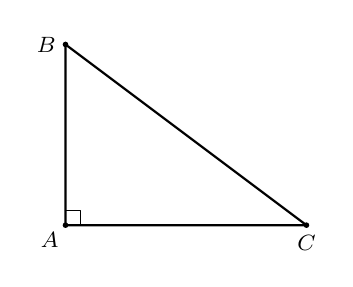
\begin{tikzpicture}[scale=0.85, >=stealth, line join=round, line cap=round, font=\footnotesize]
  \coordinate (A) at (0, 0);
  \coordinate (B) at (0, 2.7);
  \coordinate (C) at (3.6, 0);

  \draw[thick] (A) -- (B) -- (C) -- cycle;

  % Vuông góc tại A
  \draw (0, 0.22) -- (0.22, 0.22) -- (0.22, 0);

  \fill (A) circle (1.2pt) node[below left=-1pt] {$A$};
  \fill (B) circle (1.2pt) node[left] {$B$};
  \fill (C) circle (1.2pt) node[below] {$C$};
\end{tikzpicture}
\end{minipage}\par
\vspace{0.4mm}
\noindent\textit{Bài giải:}\dongkeHaiCot{10}
\\ \hline
\end{tabularx}

\vspace{2.2mm}

\noindent
\begin{tabularx}{\linewidth}{|X|}
\hline
\vspace{0.5mm}
\textbf{Câu 14 (0,5 điểm).} Tìm giá trị lớn nhất của biểu thức: $E = \dfrac{24}{x^2 - 6x + 15}$ với $x \in \mathbb{R}$.\par
\vspace{0.4mm}
\noindent\textit{Bài giải:}\dongkeHaiCot{6}
\\ \hline
\end{tabularx}
\end{document}
